\univlogo

{\Huge March 22}\vspace{5mm}

\section*{Producing Graduation Thesis}

I will spend four weeks starting this week to finish my graduation thesis. It consists of three parts - AGC hardware, MCU code and Android Apps. Today I will finish the first part, AGC hardware.

\subsection*{Automatic Gain Control}

Automatic gain control(AGC) is a closed-loop \href{https://en.wikipedia.org/wiki/Feedback}{feedback} regulating circuit in an \href{https://en.wikipedia.org/wiki/Amplifier}{amplifier} or chain of amplifiers, the purpose of which is to maintain a suitable signal amplitude at its output, despite variation of the signal amplitude at the input. The average or peak output signal level is used to dynamically adjust the \href{https://en.wikipedia.org/wiki/Gain_(electronics)}{gain} of the amplifiers, enabling the circuit to work satisfactorily with a greater range of input signal levels. It is used in most \href{https://en.wikipedia.org/wiki/Radio_receiver}{radio receivers} to equalize the average volume (\href{https://en.wikipedia.org/wiki/Loudness}{loudness}) of different radio stations due to differences in received \href{https://en.wikipedia.org/wiki/Signal_strength}{signal strength}, as well as variations in a single station's radio signal due to \href{https://en.wikipedia.org/wiki/Fading}{fading}. Without AGC the sound emitted from an \href{https://en.wikipedia.org/wiki/Amplitude_modulation}{AM} \href{https://en.wikipedia.org/wiki/Radio}{radio} receiver would vary to an extreme extent from a weak to a strong signal; the AGC effectively reduces the volume if the signal is strong and raises it when it is weaker. In a typical receiver the AGC feedback control signal is usually taken from the \href{https://en.wikipedia.org/wiki/Detector_(radio)}{detector} stage and applied to control the gain of the IF or RF amplifier stages.

\rightline{--- From \href{https://en.wikipedia.org/wiki/Automatic_gain_control}{Wikipedia}}

\subsection*{AGC IC selection}

I use a low noise, voltage-controlled amplifier AD603 to design peripheral circuit:

\begin{figure}[H]
\centering
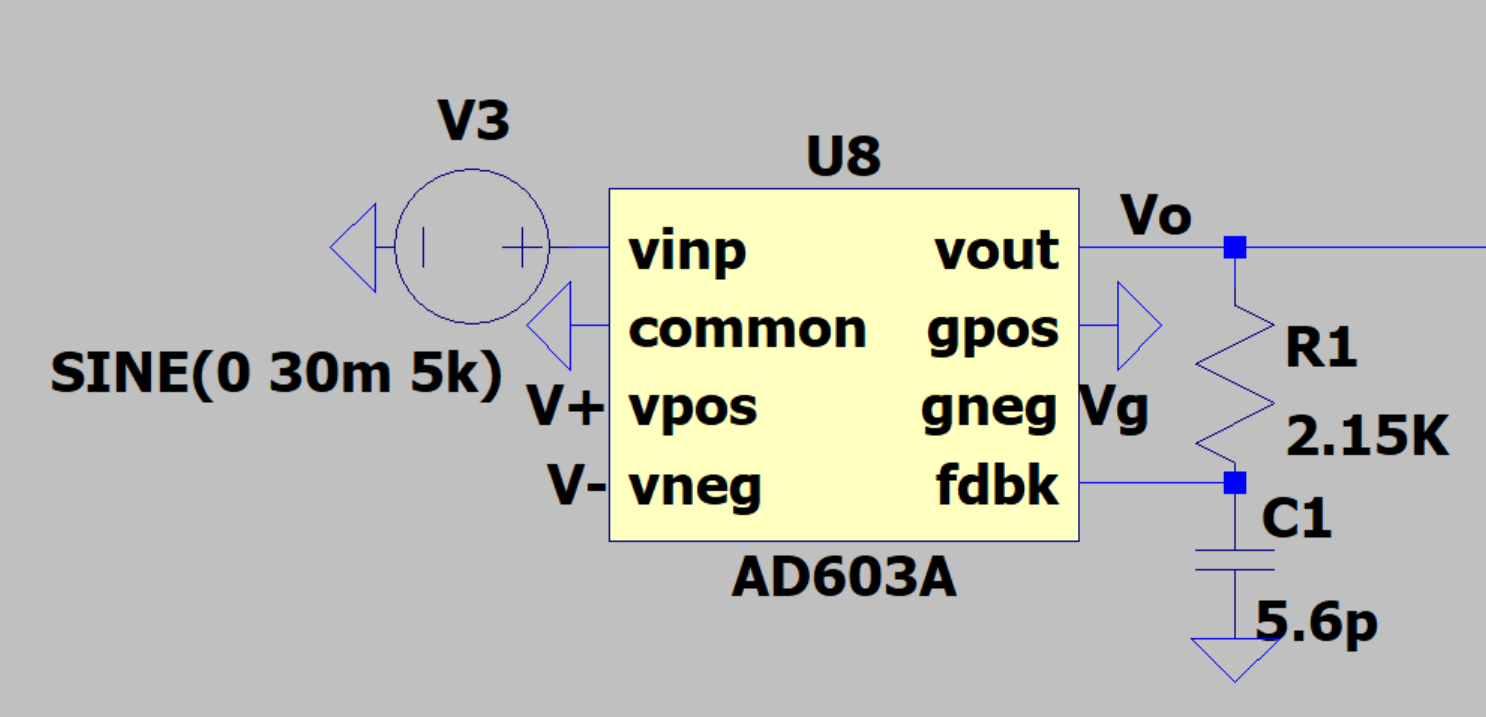
\includegraphics[width=0.8\textwidth]{./2023Mar/AD603.png}
\caption{AD603 Circuit}
\label{AD603}
\end{figure}

$V_g$ is the voltage signal that is fed back from the rear stage to control the gain.

\subsection*{Envelope Detection}

For the AGC output signal $V_o$, an envelope detector is required to obtain the amplitude information. The following envelope detector circuit is used:

\begin{figure}[H]
\centering
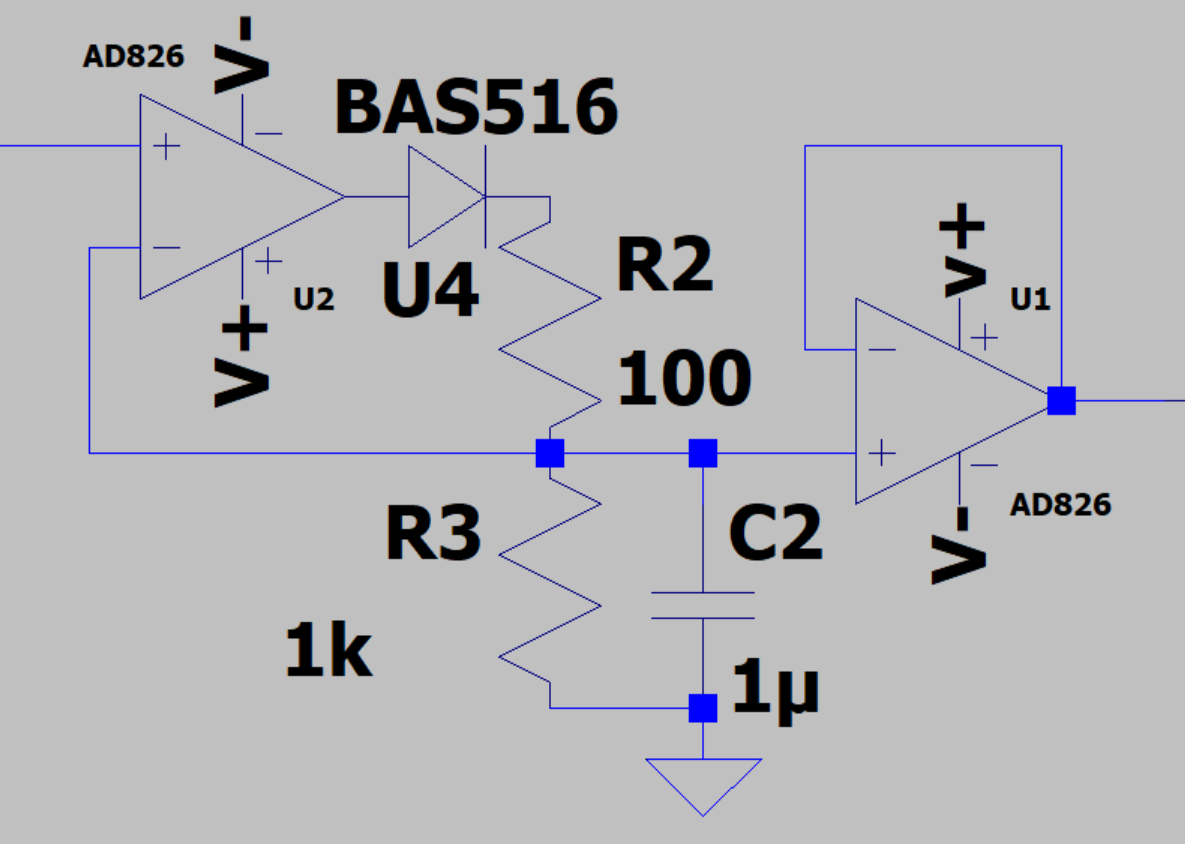
\includegraphics[width=0.6\textwidth]{./2023Mar/EnvolopDetect.png}
\caption{Envolop Detect}
\label{EnvolopDetect}
\end{figure}

As is shown above, the amplitude info can be dectected by the OPA at the first stage and the voltage will be applied across the capacitor $C2$. $R3$ and $C2$ form a RC circuit. The circuit can discharge through R3 when the signal amplitude drops. The rate of discharge depends on the time constant $\tau=R3\cdot C2$. The time constant should not be too large or the discharge rate will be too slow as is shown below:

\begin{figure}[H]
\centering
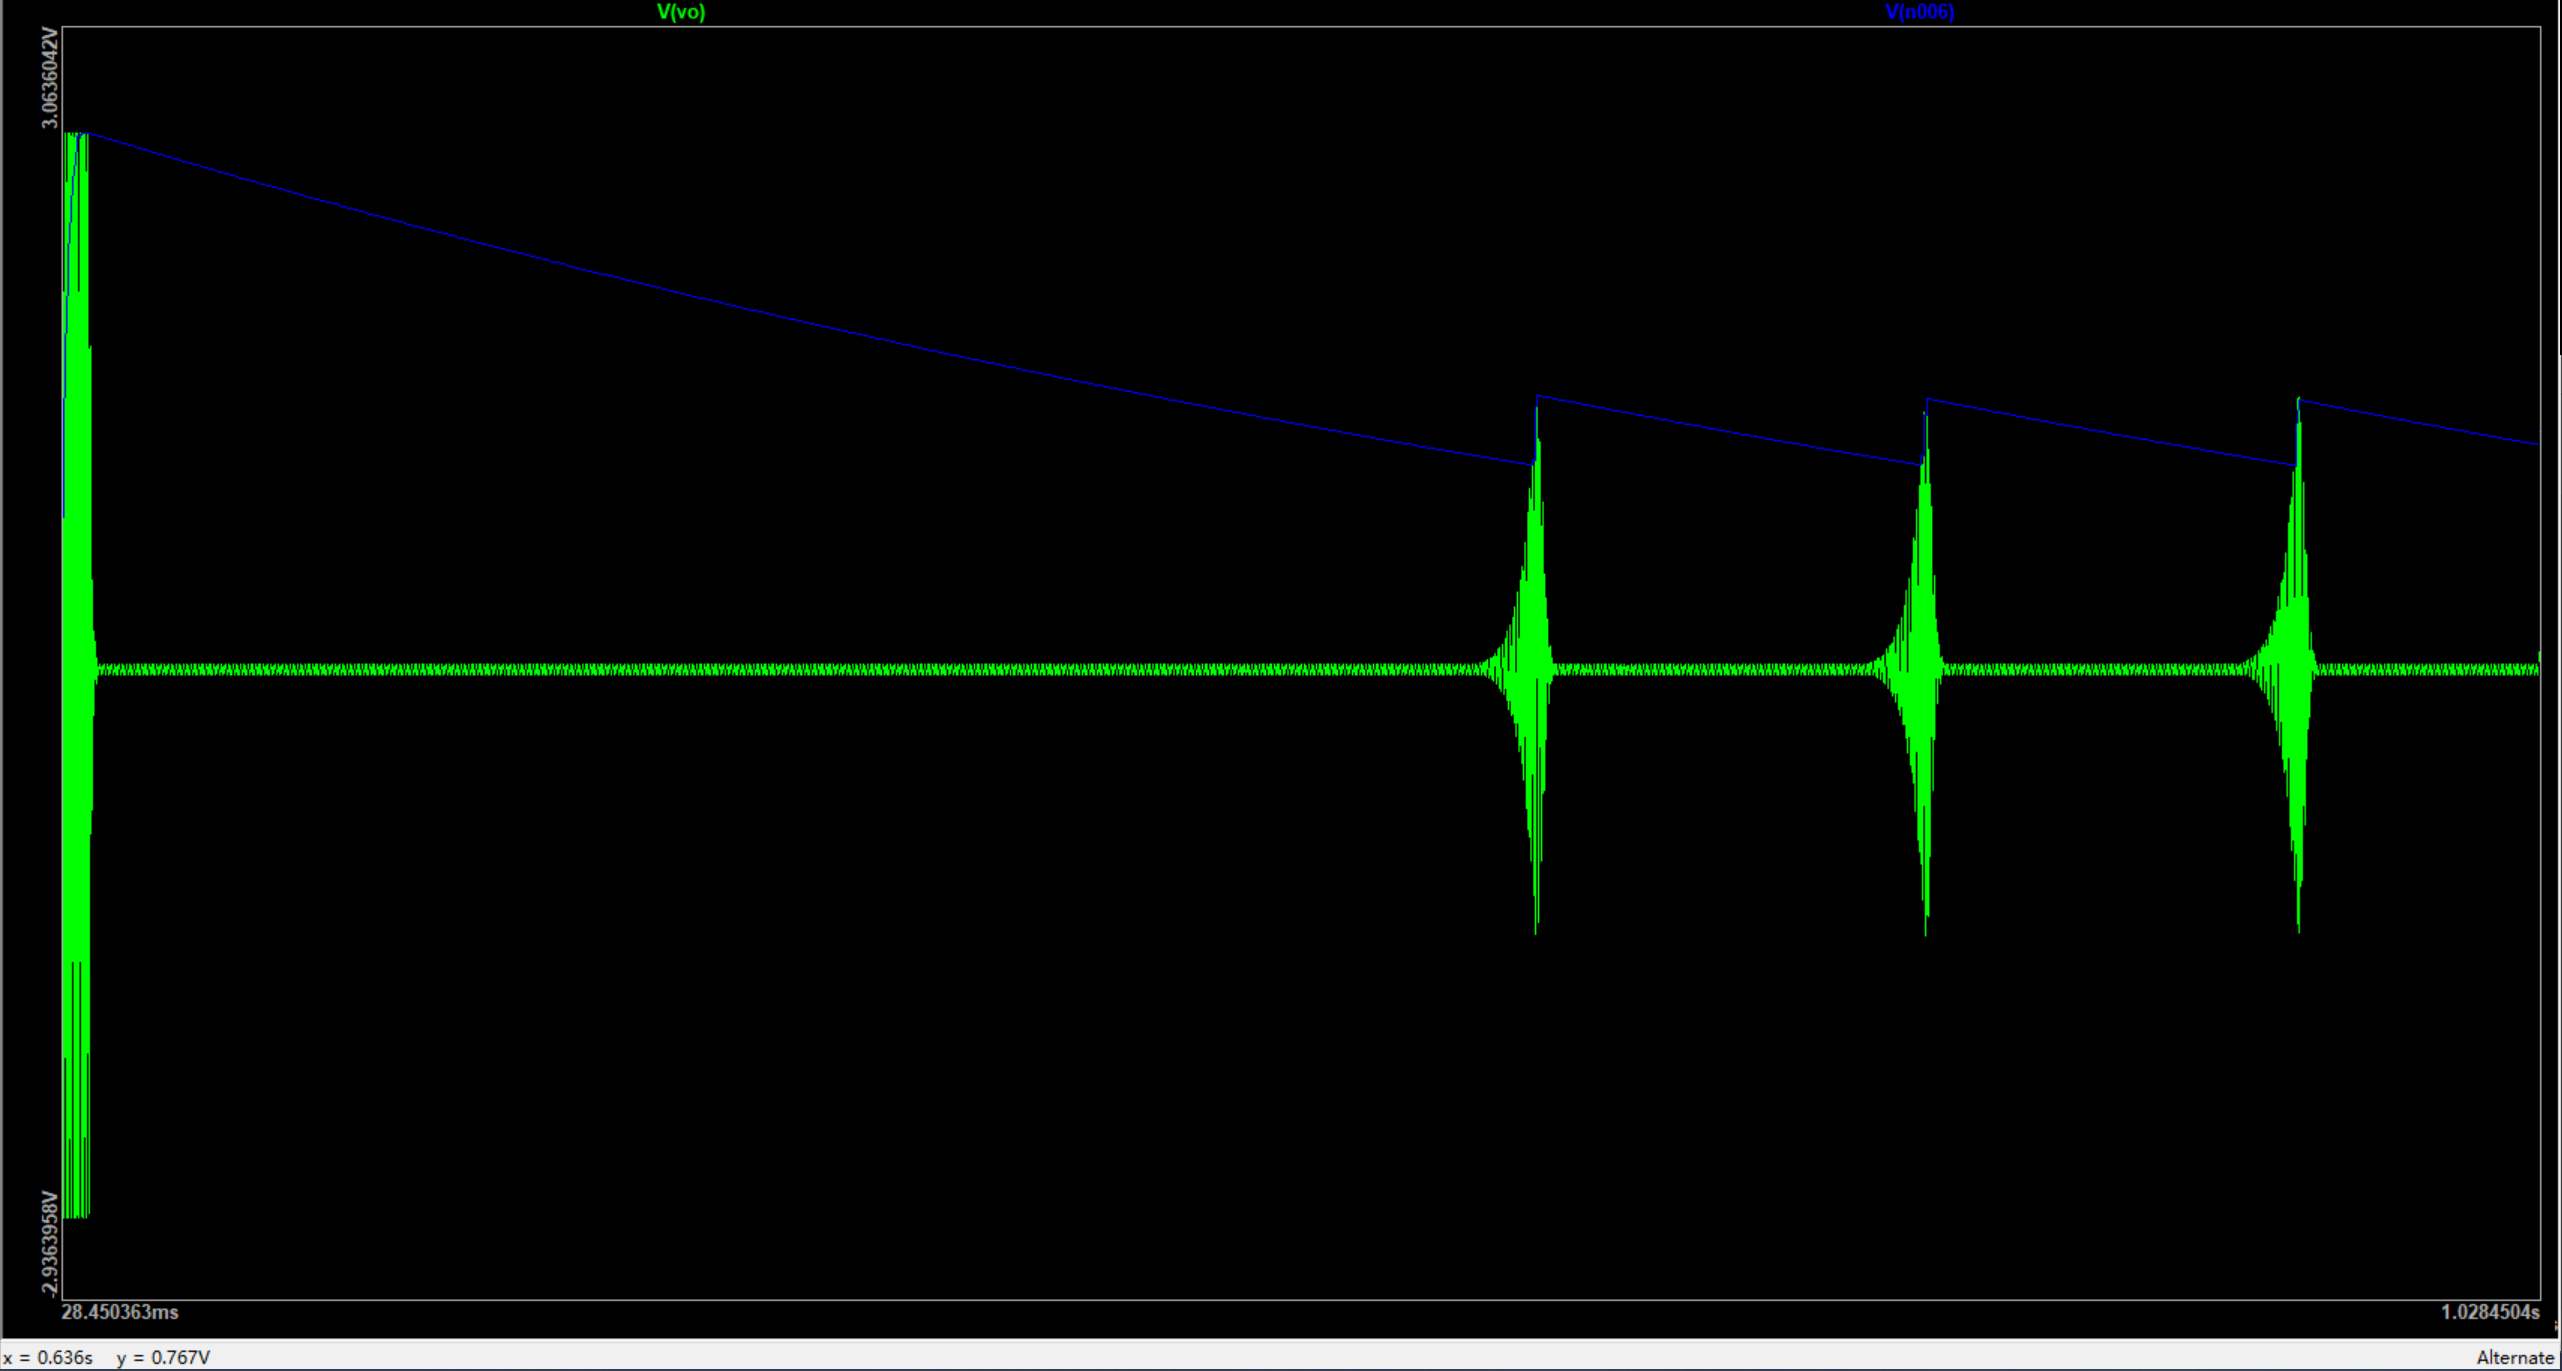
\includegraphics[width=0.8\textwidth]{./2023Mar/WaveEnvDectErr.png}
\caption{The discharge rate is too slow}
\label{WaveEnvDectErr}
\end{figure}

We need to set up an appropriate time constant $\tau$. The correct graph line is shown below:

\begin{figure}[H]
\centering
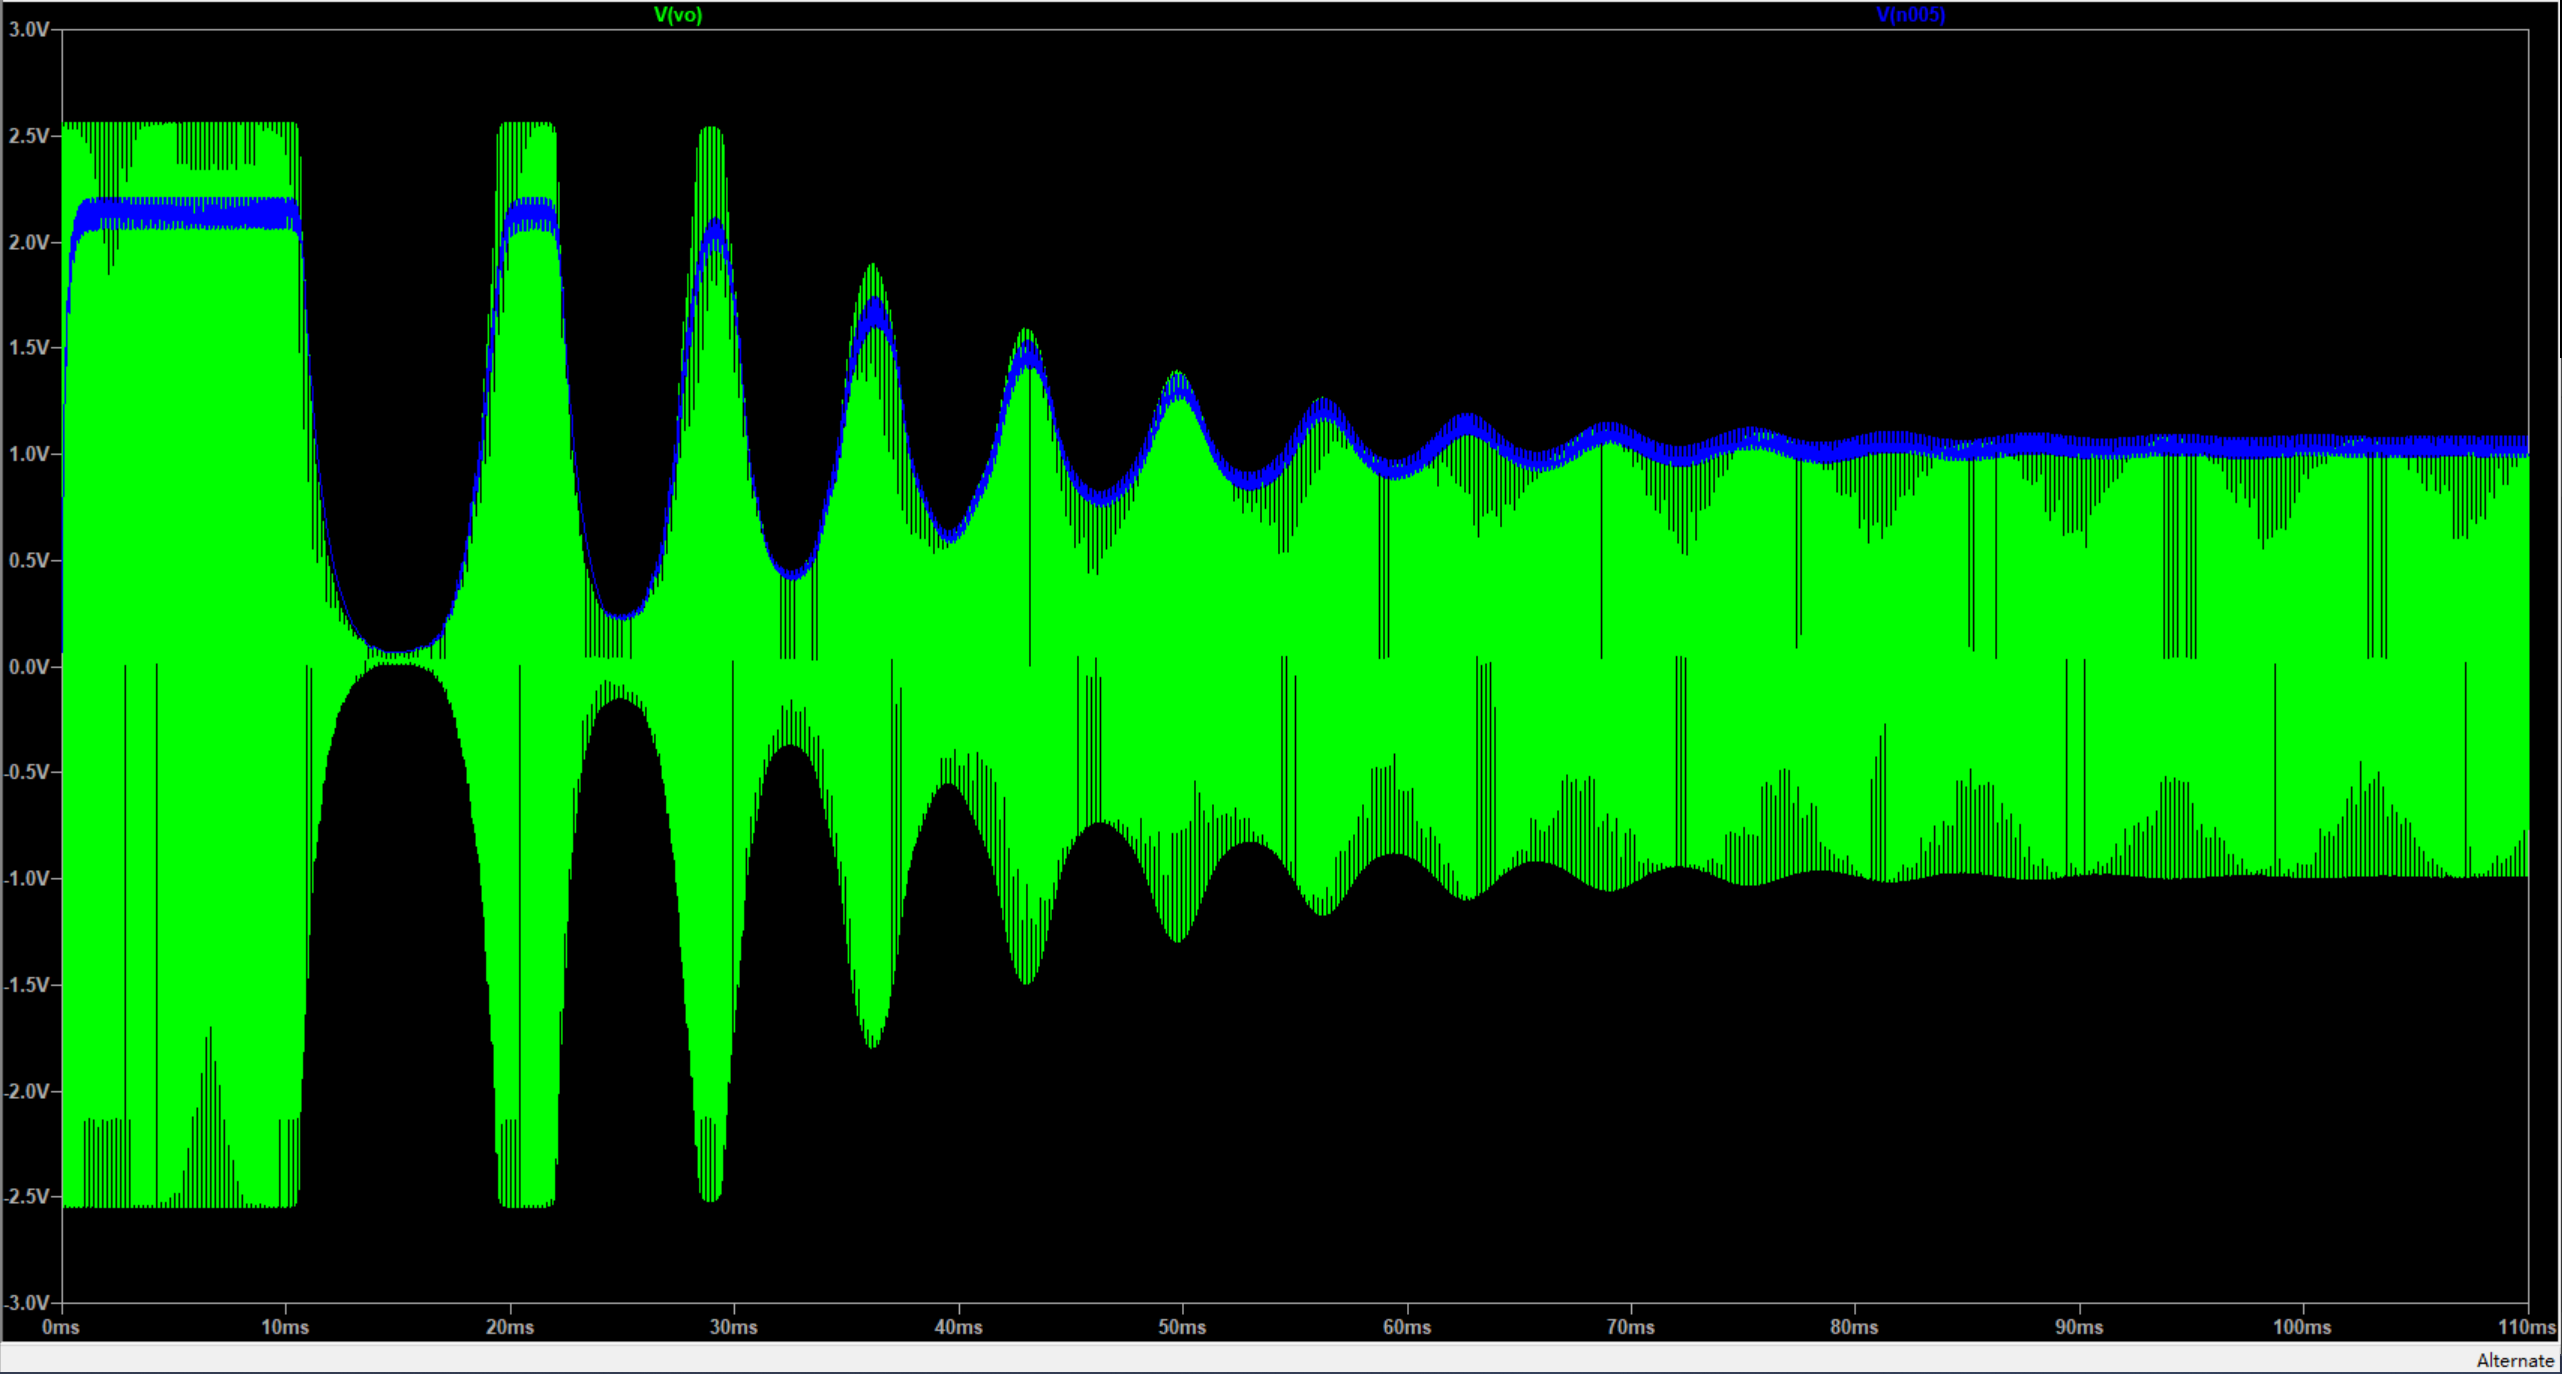
\includegraphics[width=0.8\textwidth]{./2023Mar/WaveEnvDect.png}
\caption{Correct envelope detect graph line}
\label{WaveEnvDect}
\end{figure}

It can be clearly seen that the circuit accurately detects the envelope signal output by the AGC, and under the action of the post-stage feedback, after a period of oscillation, the output signal is controlled within a reasonable amplitude range.

\subsection*{Calculate the feedback signal}

After obtaining the amplitude of the AGC output signal, we can obtain a reasonable AGC control signal $Vg$ through the linear operation of the operational amplifier.

\begin{figure}[H]
\centering
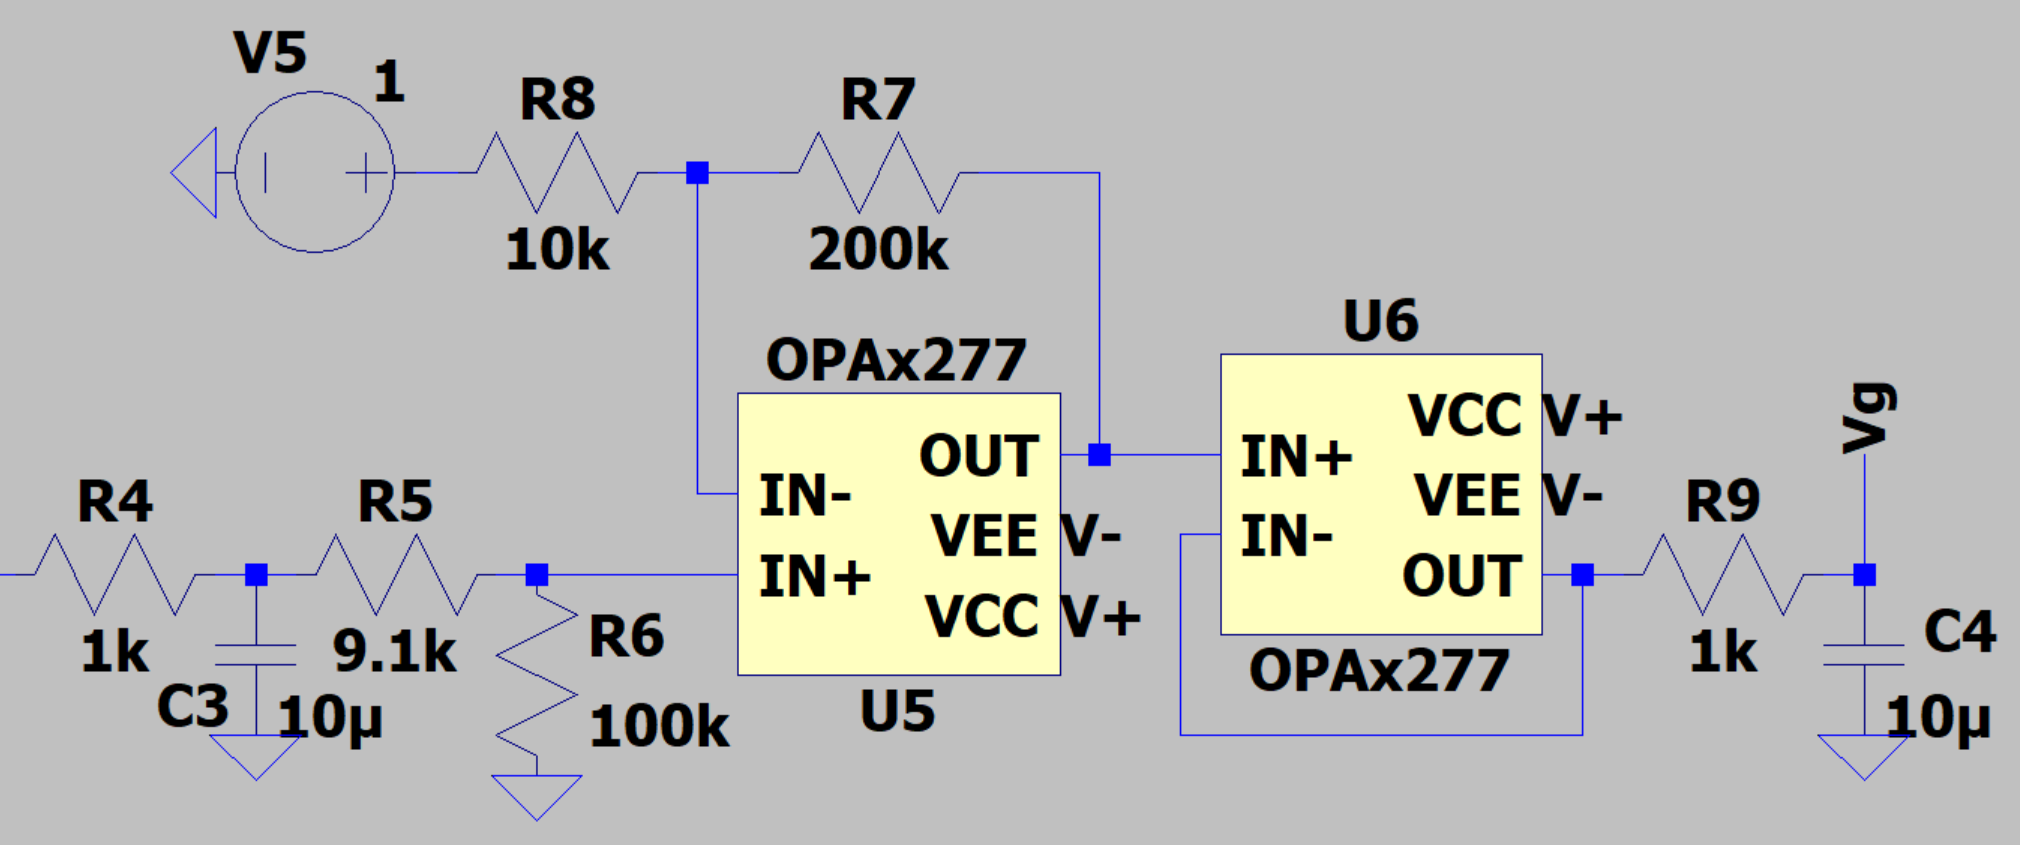
\includegraphics[width=1\textwidth]{./2023Mar/difference.png}
\caption{Linear operation of the operational amplifier}
\label{difference}
\end{figure}


In the schematic, we conduct \textbf{high-pass filter} and \textbf{divided voltage} on the result of envelope detection, and then calculate the difference with the standard voltage reference, and feed back the result $V_g$ to the control terminal of AD603.

\subsection*{Add DC bias}

Since the analog input pin of the MCU has a certain input voltage range limitation, we need to add a DC bias to the AC signal output by the AGC. Here we use a rail-to-rail OPA OPA340.

\begin{figure}[H]
\centering
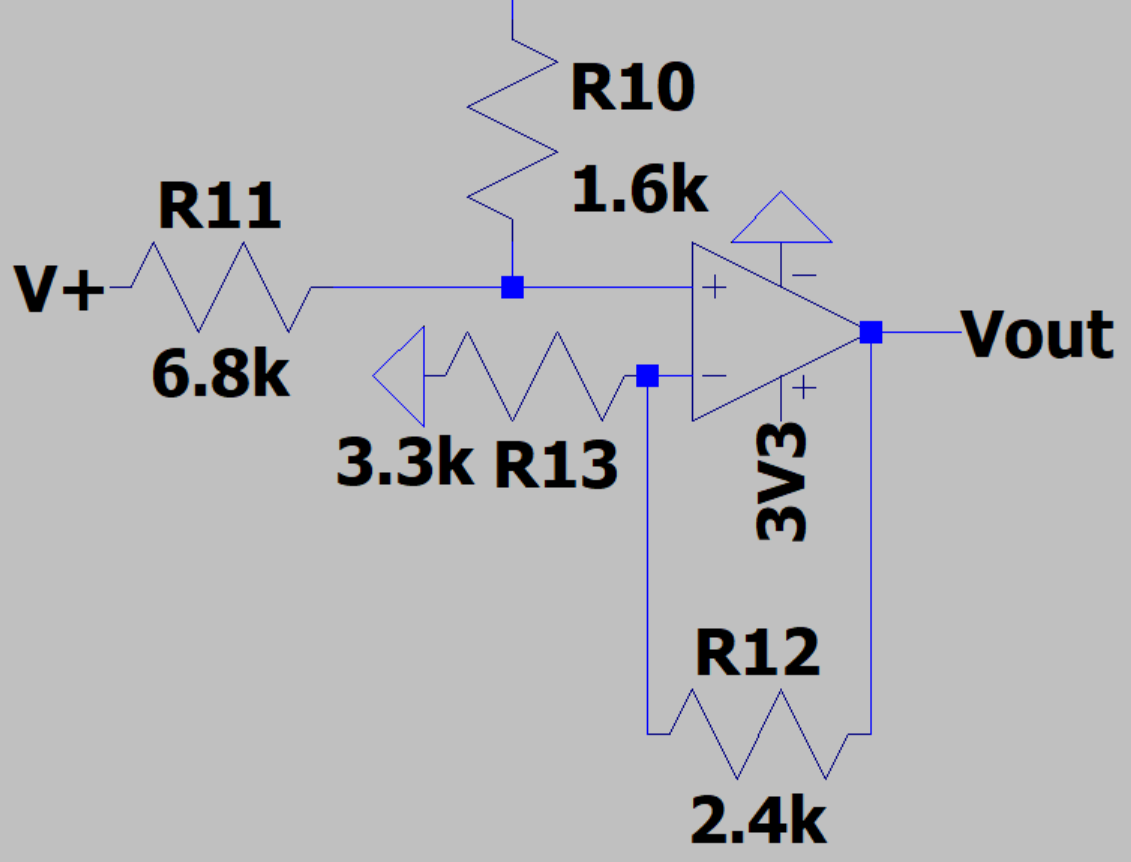
\includegraphics[width=0.8\textwidth]{./2023Mar/AddDC.png}
\caption{Add DC bias}
\label{Add DC}
\end{figure}

The waveforms before and after adding DC bias are as follows:

\begin{figure}[H]
\centering
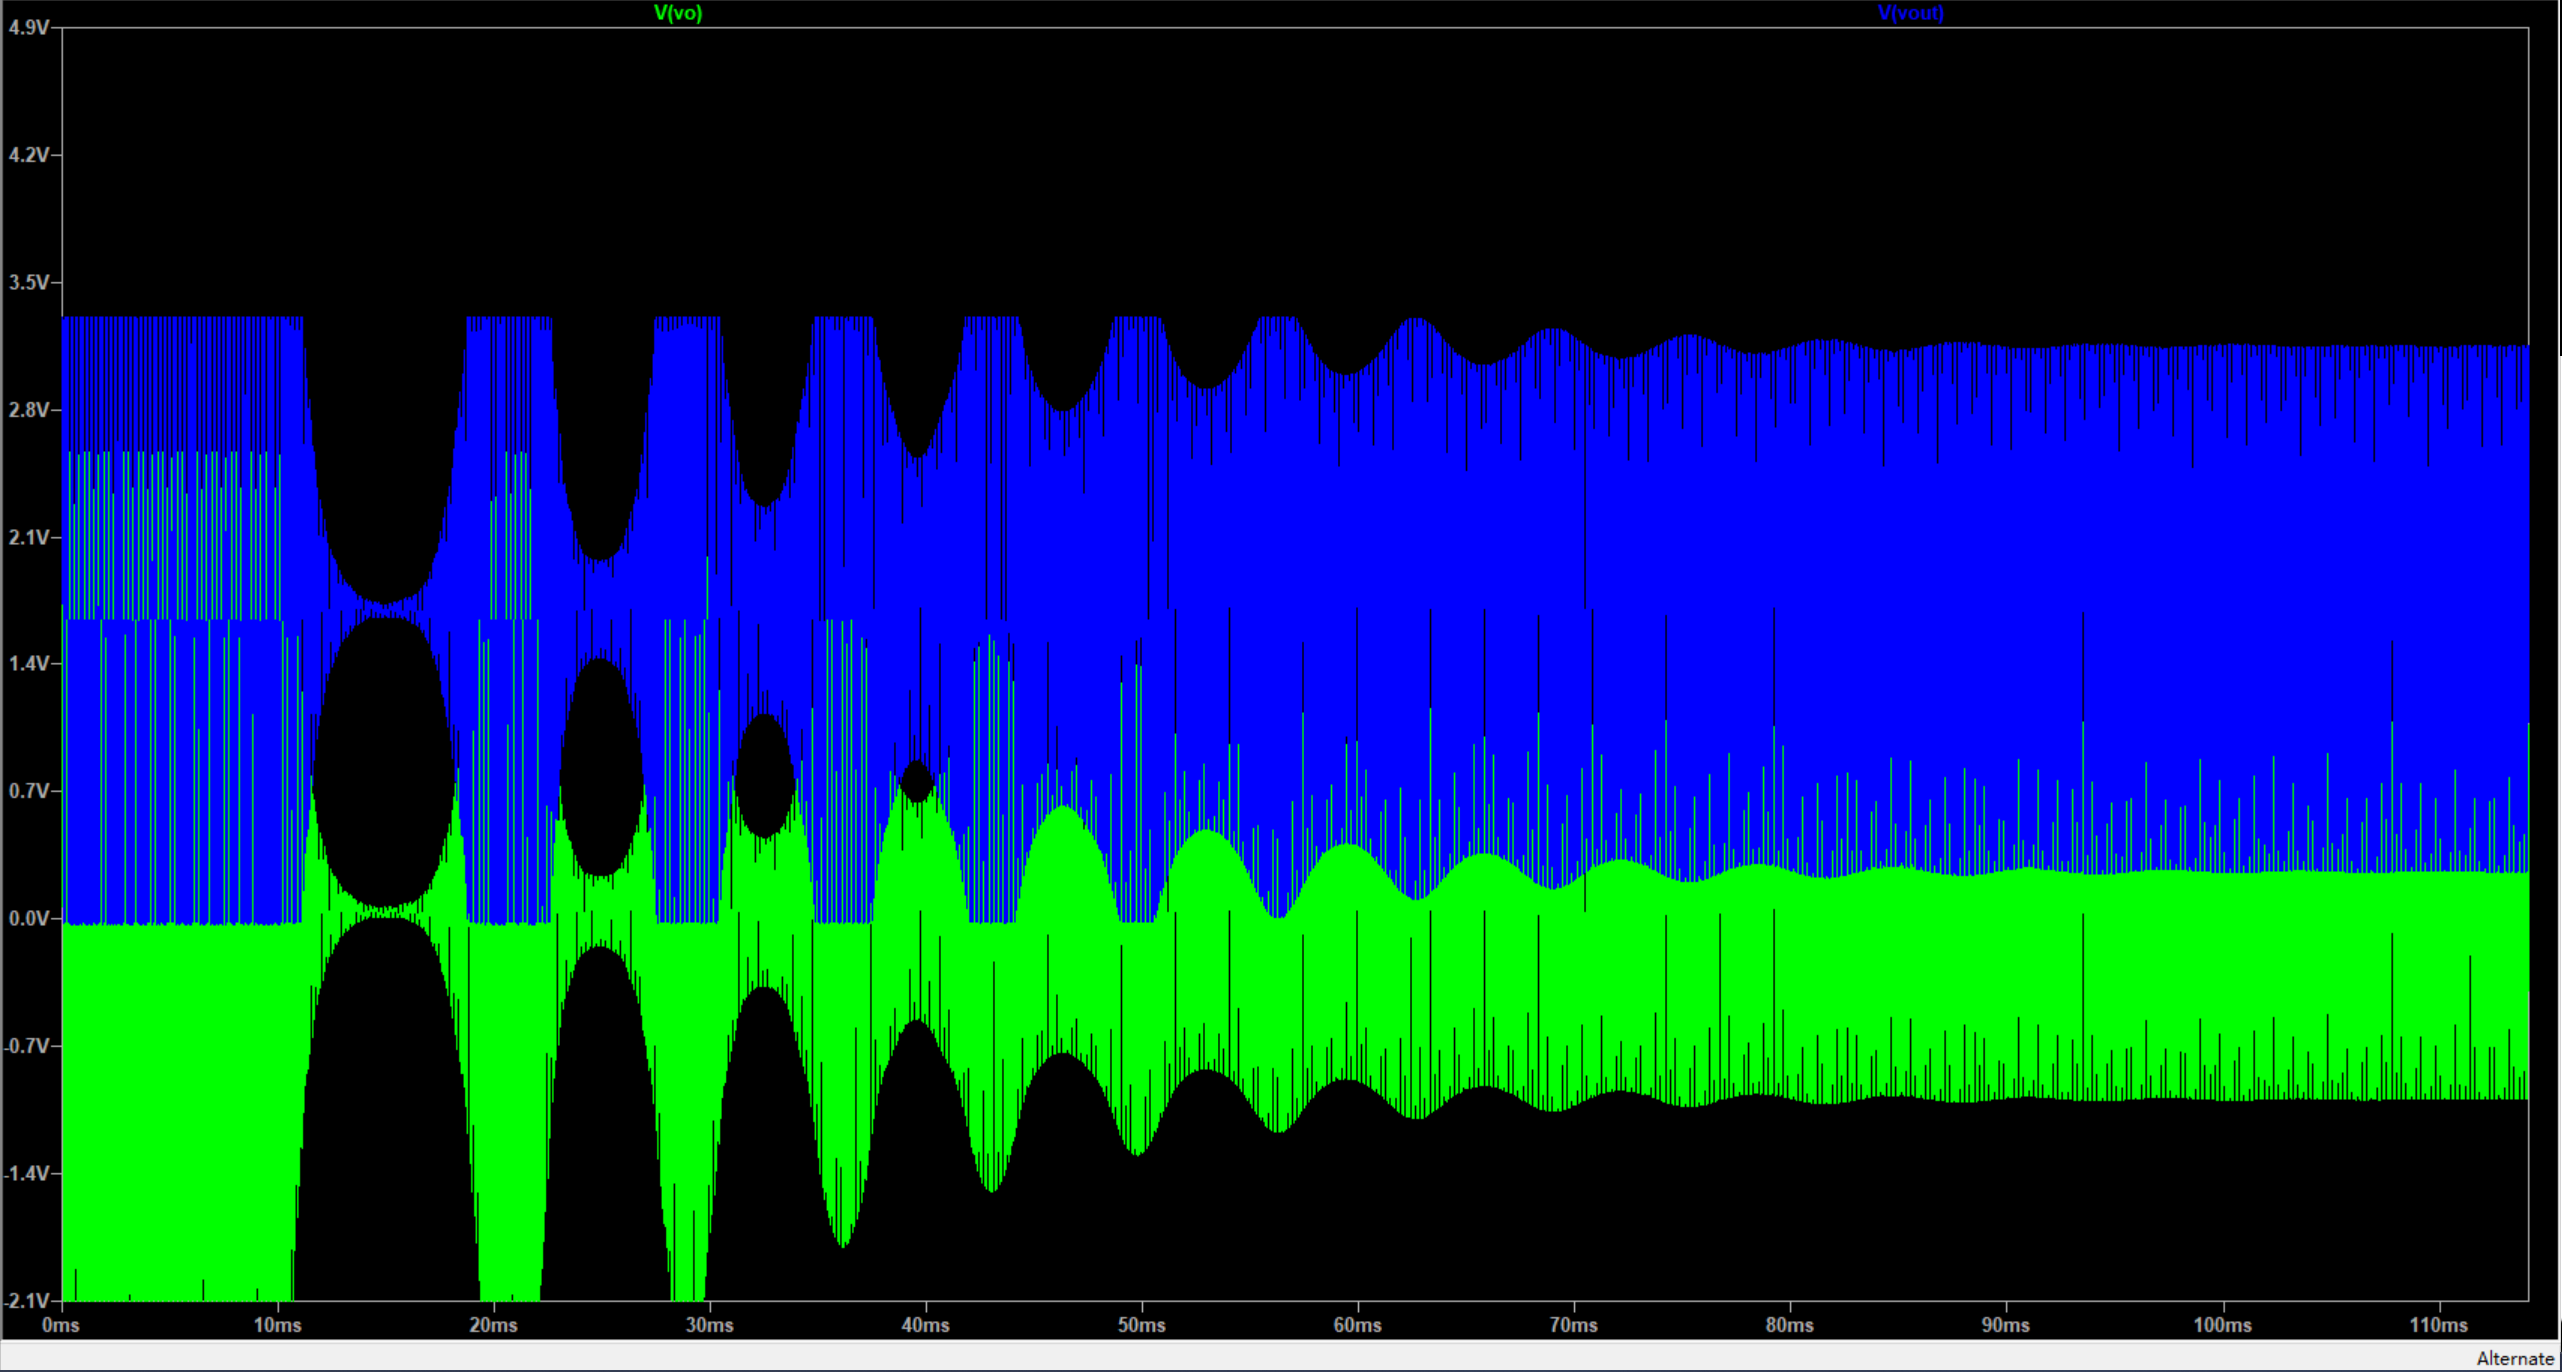
\includegraphics[width=0.8\textwidth]{./2023Mar/WaveAddDC.png}
\caption{Waveforms before and after adding DC bias}
\label{WaveAddDC}
\end{figure}

\subsection*{System}

We use LTspice, a free simulation tool provided by ADI, to build the simulation circuit.

\begin{figure}[H]
\centering
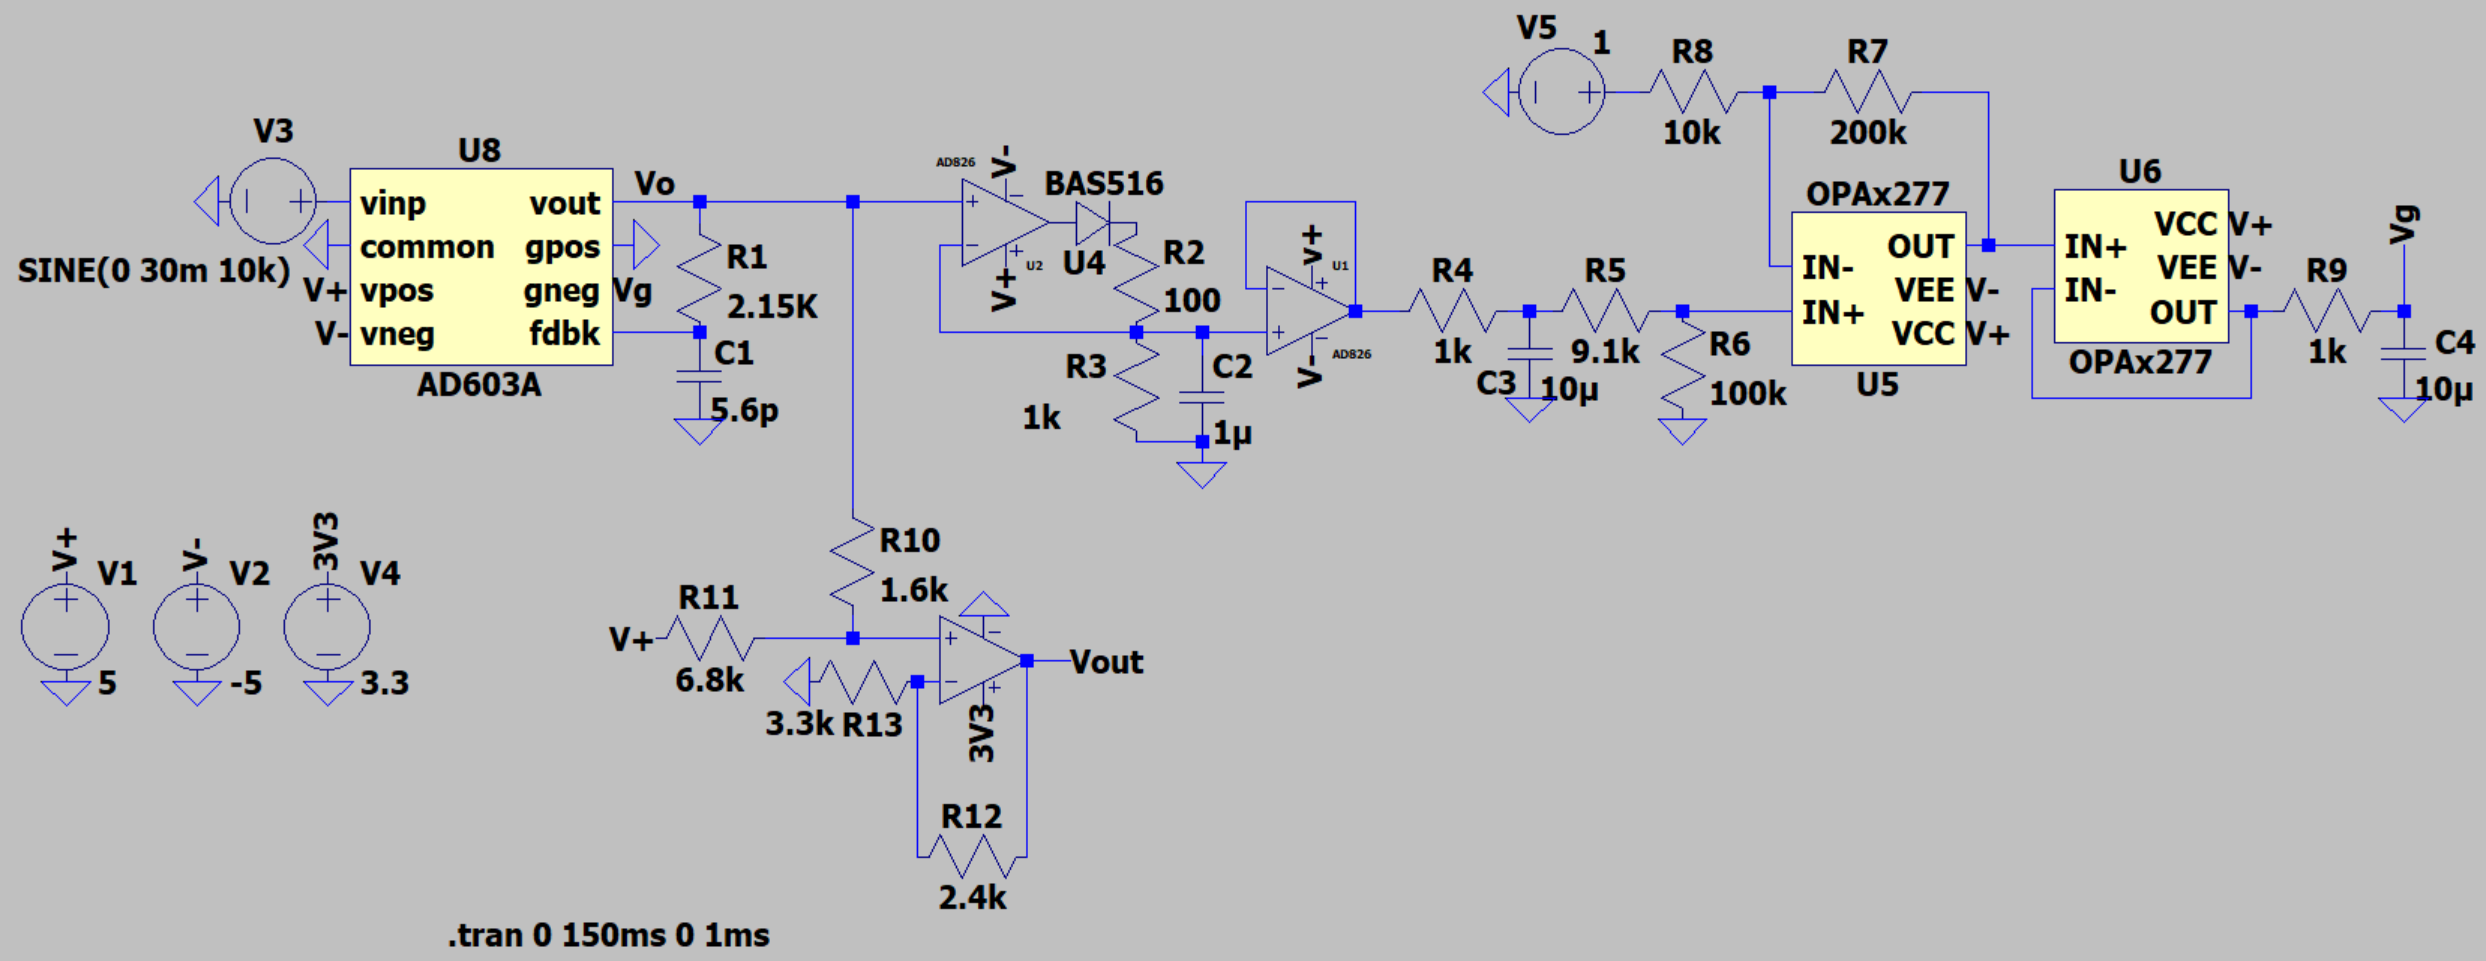
\includegraphics[width=1\textwidth]{./2023Mar/system.png}
\caption{The whole system}
\label{system}
\end{figure}

Set the simulation type to transient response simulation, with a total duration of 150ms and a step of 1ms. We can see the waveform of each node as follows:

\begin{figure}[H]
\centering
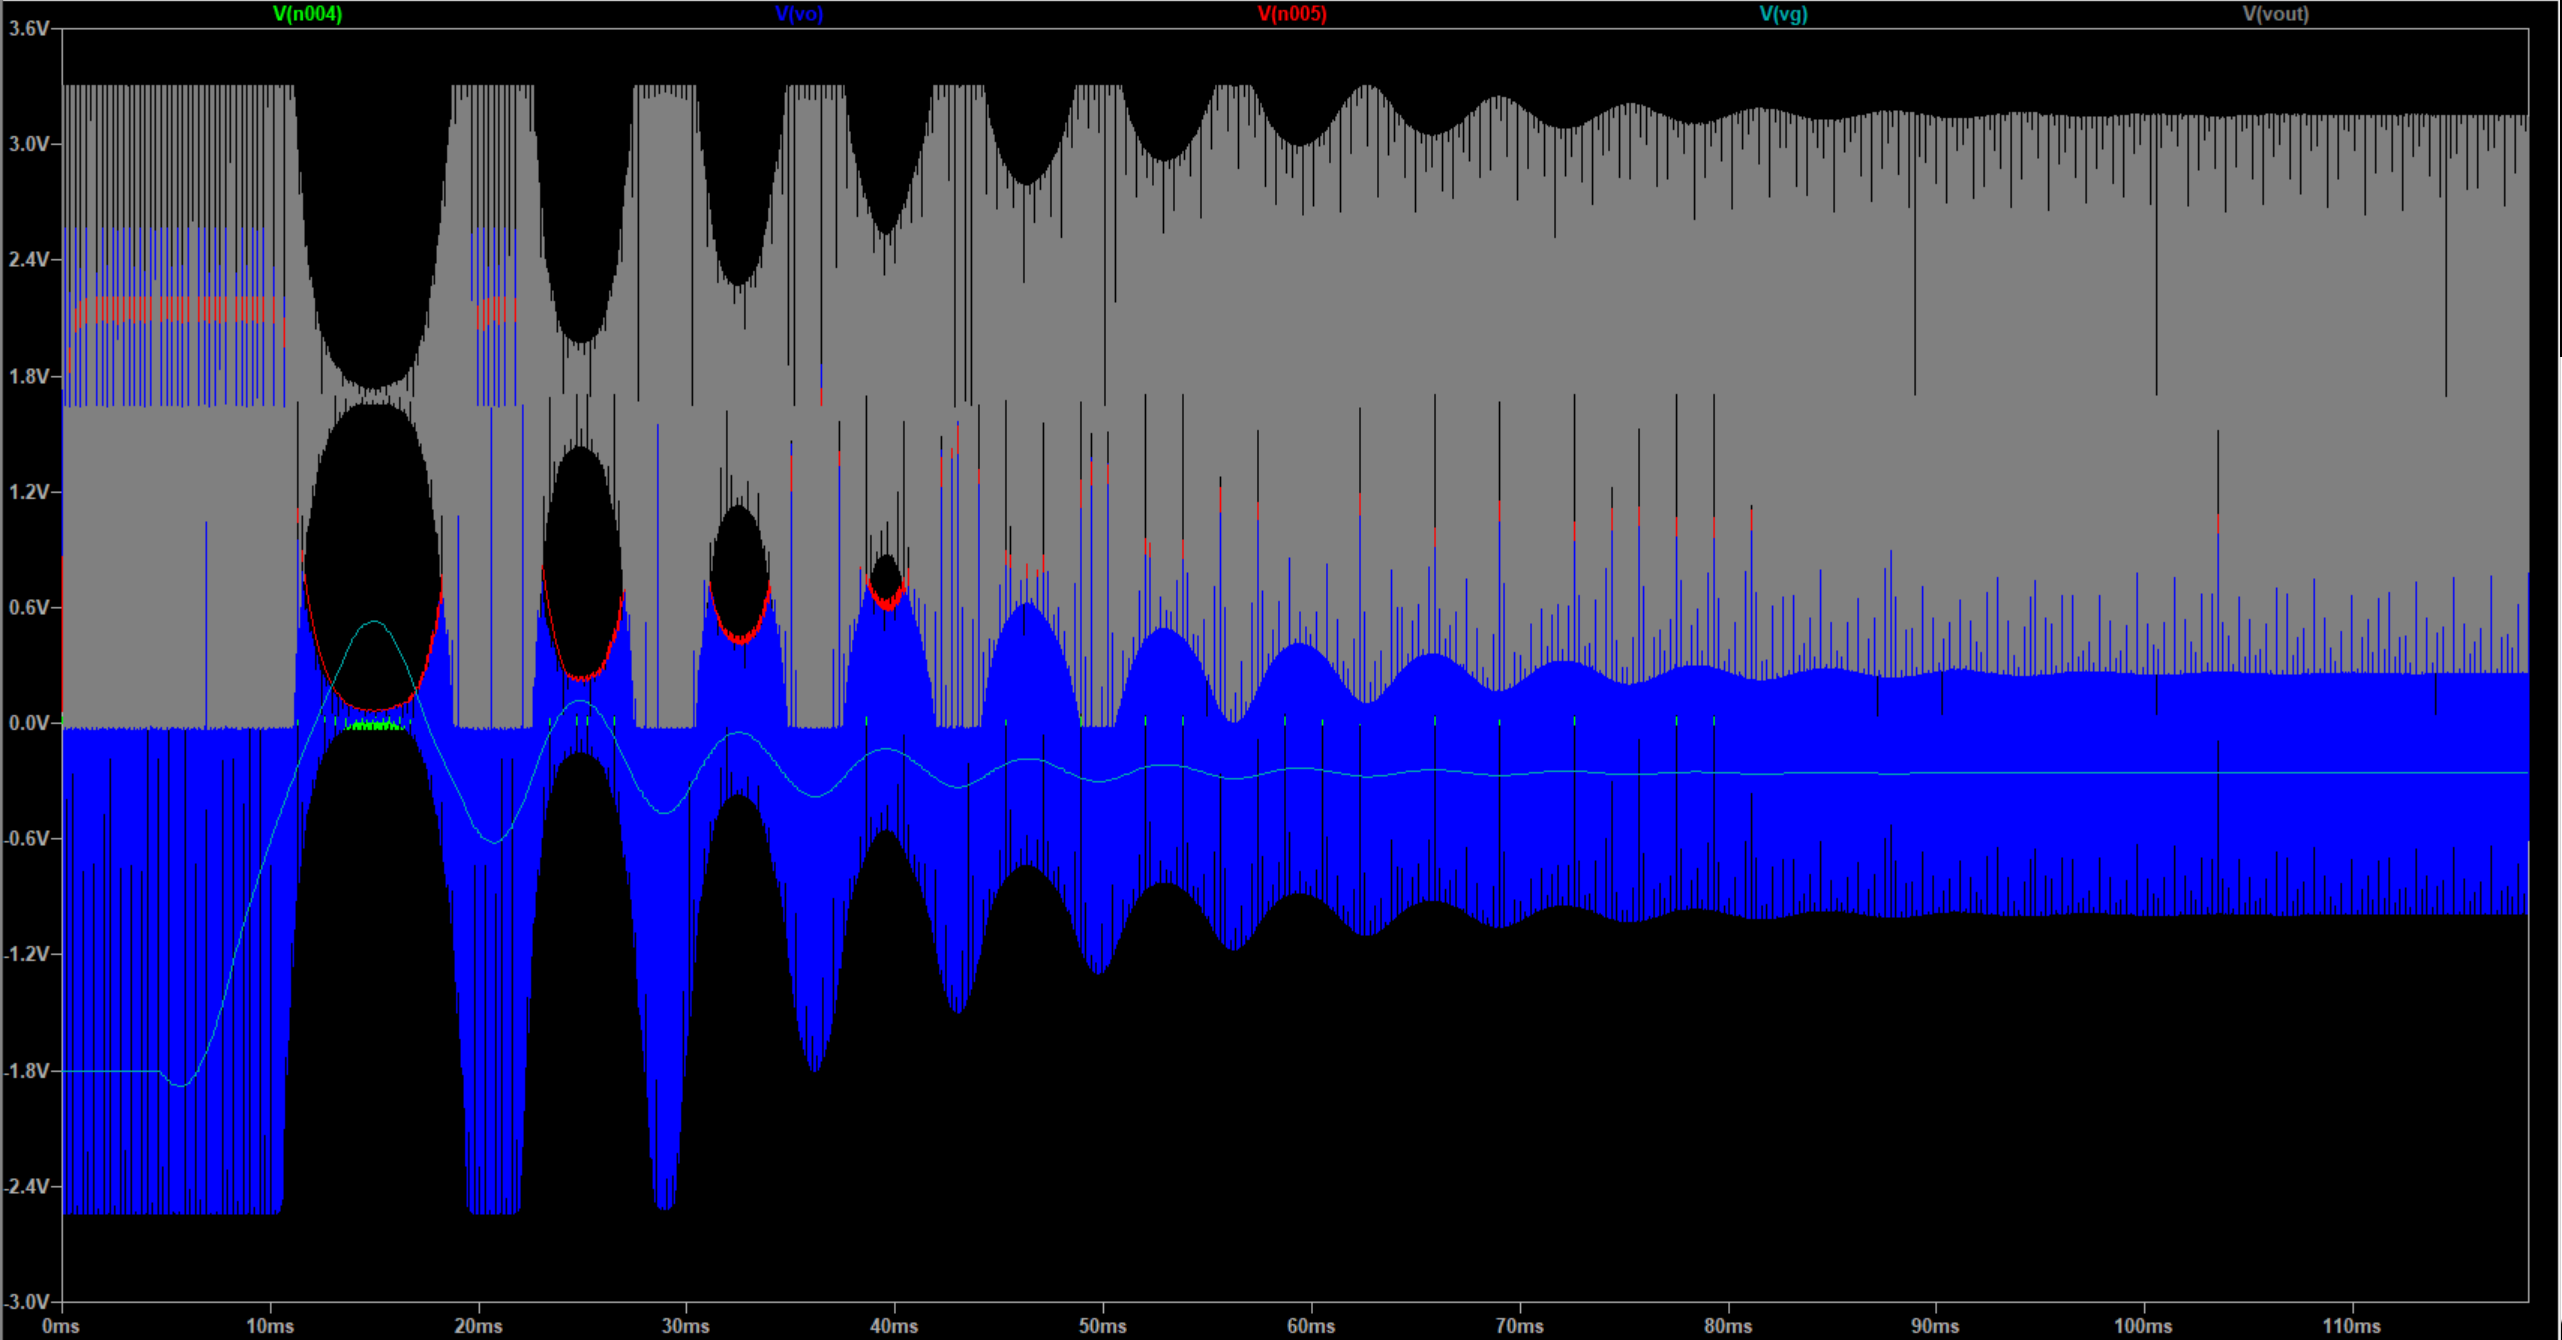
\includegraphics[width=1\textwidth]{./2023Mar/WaveAll.png}
\caption{Waveform of each node}
\label{WaveAll}
\end{figure}

After the system become stable, the details are shown below:
\begin{figure}[H]
\centering
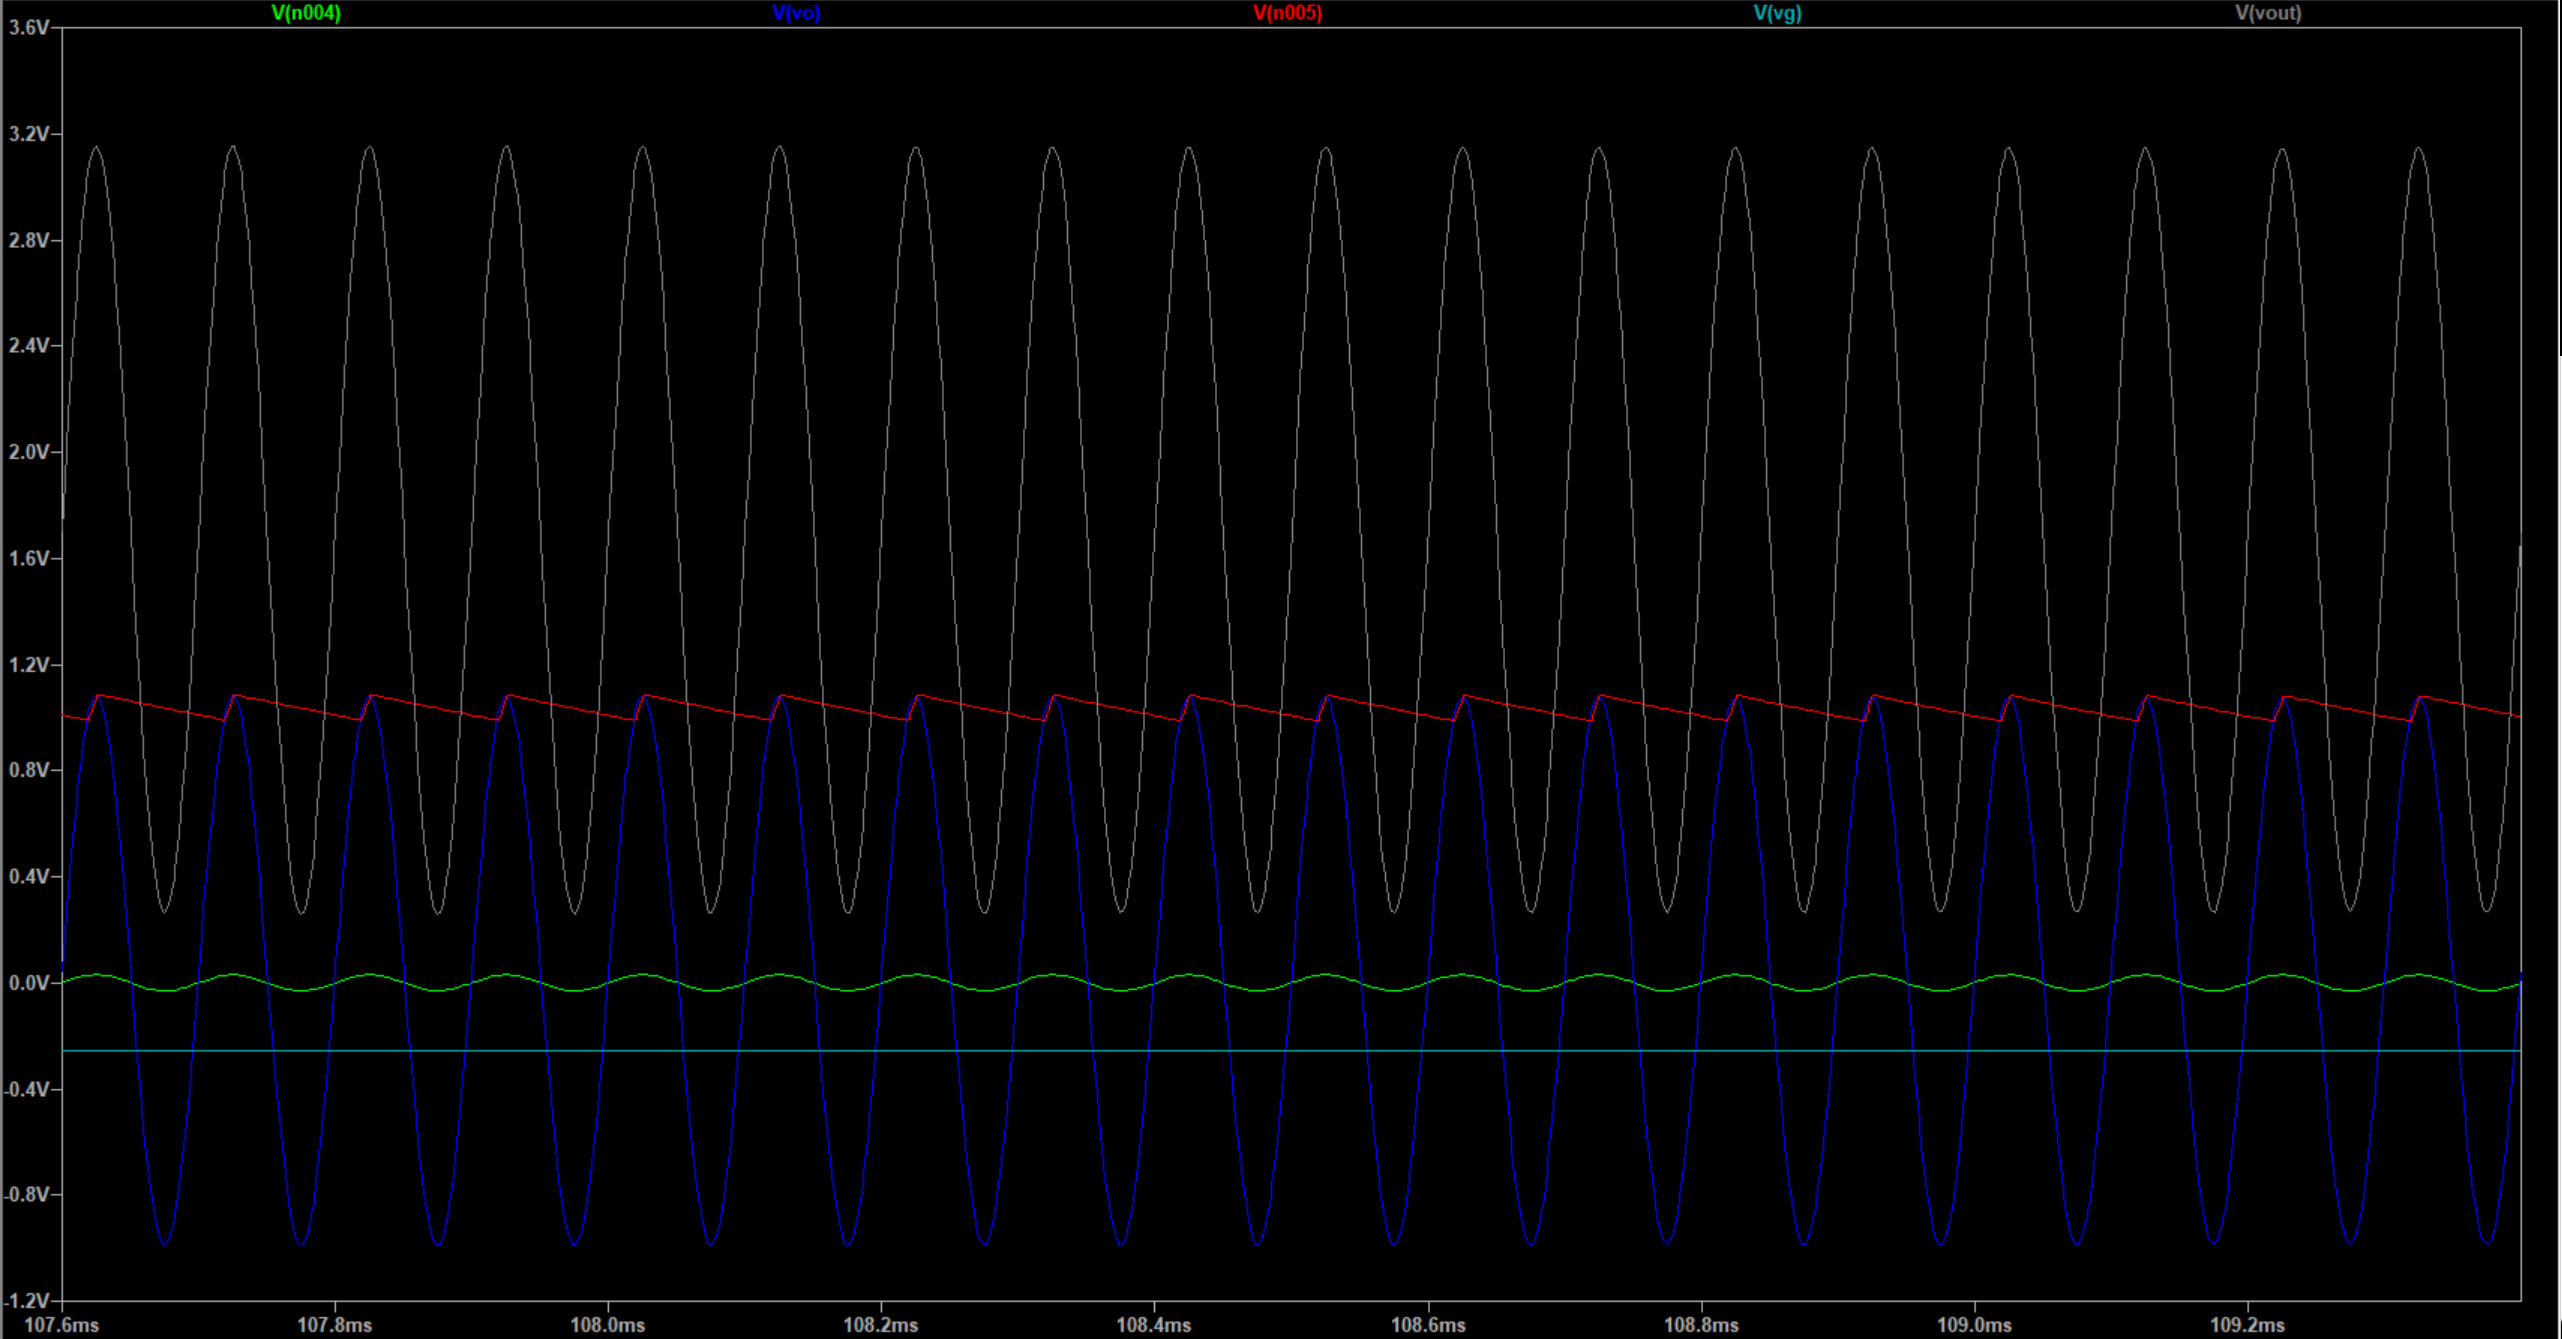
\includegraphics[width=1\textwidth]{./2023Mar/WaveAllLocal.png}
\caption{Details}
\label{WaveAllLocal}
\end{figure}

The white line is the final output result.
